\clearpage
\subsection{premi/client/infographicEditor}
\begin{figure}[h]
\begin{center}
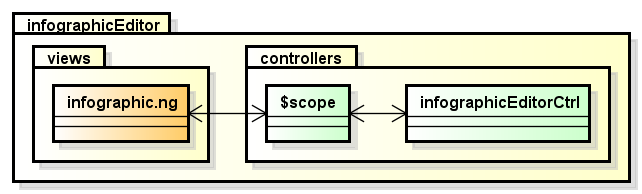
\includegraphics[scale=0.55]{img/diapkg/infographicEditor.png}
\caption{Diagramma del package premi/client/infographicEditor}
\end{center}
\end{figure}



%-------  diagramma di un template %
\subsubsection{premi/client/infographicEditor/views/infographic.ng}

\begin{description}
%-------  descrizione del template%
\item[Descrizione] \hfill \\
	Template della vista associata allo \textit{\$scope} di \textit{infographicEditorCtrl}. Fornisce tutti gli strumenti necessari alla modifica dell'infografica della presentazione, tra cui:
	\begin{itemize}
			\item aggiunta e rimozione dei frame creati finora dall'utente
			\item inserimento, modifica e rimozione di immagini, shape, e testo
			\item spostamento e ridimensionamento di frame, immagini, shape  e testo all'interno dell'infografica
	\end{itemize}
\end{description}



















%-------  diagramma della classe%
\subsubsection{premi/client/infographicEditor/controllers/infographicEditorCtrl}
\begin{figure}[h]
\begin{center}
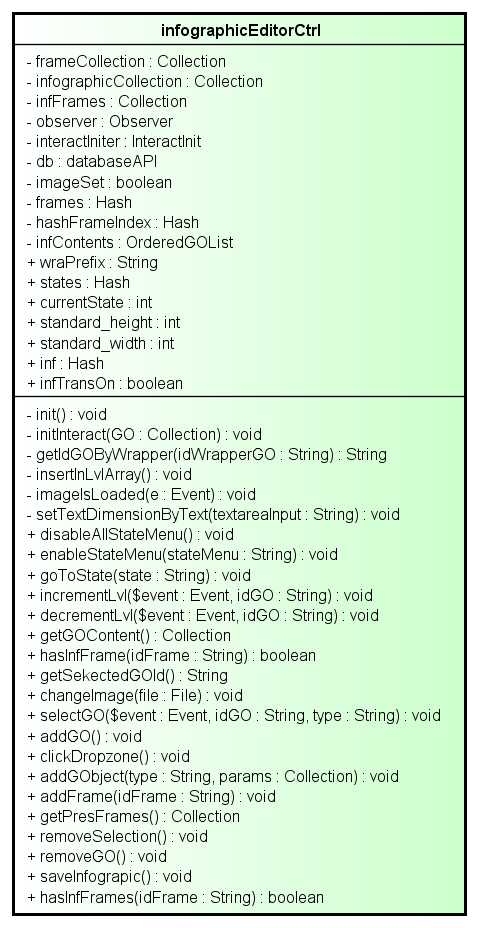
\includegraphics[scale=0.55]{img/diacla/infographicEditorCtrl.png}
\caption{Diagramma della classe premi/client/infographicEditor/controllers/infographicEditorCtrl}
\end{center}
\end{figure}


\begin{description}
%-------  descrizione della classe%
\item[Descrizione] \hfill \\
	Questo controller crea lo \$scope associato alla vista generata da \textbf{infographic.ng}, fornendo i dati e i metodi necessari per consentire all'utente di creare e modellare l'infografica di una presentazione, inserendo o rimuovendo frame e altri oggetti grafici al suo interno.
	
	
	
%-------  lista delle classi associate%	
\item[Dipendenze] \hfill \\
	\begin{itemize}
		\item \textbf{premi/client/presentation/lib/databaseAPI}: per l'accesso ai metodi che interagiscono con il database
		\item \textbf{premi/client/editor/lib/InteractInit}: per collegarsi alla libreria esterna Interact.js e visualizzare oggetti grafici e frame
		\item \textbf{premi/client/editor/lib/Observer}: fornisce agli oggetti che compongono l'infografica un observer per l'aggiornamento in tempo reale delle modifiche apportate ad essi
		\item \textbf{premi/client/editor/lib/Infographic}: per la creazione e modifica dell'infografica
	\item \textbf{premi/client/presentation/lib/OrderedGOList}: per la gestione degli oggetti grafici contenuti all'interno dell'infografica
	\end{itemize}
	
	
%-------  lista degli Attributi%	
\item[Attributi] \hfill \\
	\begin{description}
		\item[\textbf{- frameCollection : Collection 			}] \hfill \\
			Collezione di MongoDB di tutti i frame creati dall'utente per la presentazione che sta modificando
		\item[\textbf{- infographicCollection : Collection			}] \hfill \\
			Collezione di MOngoDB. Contiene gli attributi dell'infografica associata alla presentazione che l'utente intende modificare
		\item[\textbf{- infFrames : Collection 			}] \hfill \\
			Collezione di MongoDB dei frames finora inseriti all'interno dell'infografica
		\item[\textbf{- observer : Observer 			}] \hfill \\
			Oggetto Observer da collegare agli oggetti che compongono l'infografica
		\item[\textbf{- interactIniter : InteractInit			}] \hfill \\
			Serve a inizializzare la libreria Interact.js per la visualizzazione degli oggetti grafici
		\item[\textbf{- db : databaseAPI			}] \hfill \\
			Oggetto creato per l'utilizzo dei metodi statici contenuti al suo interno, che permettono al controller di accedere al server per il salvataggio delle modifiche apportate 
		\item[\textbf{- frames : Hash			}] \hfill \\
			Lista di frames inseriti finora nell'infografica, composta da \textit{frame\_id} : \textit{collezione di attributi}
		\item[\textbf{- hashFrameIndex : Hash			}] \hfill \\
			Lista di codici identificativi dei frame inseriti finora nell'infografica, associati alla loro posizione all'iterno di frameCollection
		\item[\textbf{- infContents : OrderedGOList			}] \hfill \\
			Lista ordinata degli oggetti grafici inseriti finora all'interno dell'infografica
		\item[\textbf{+ wraPrefix : String			}] \hfill \\
			Prefisso del codice identificativo dei contenitori degli oggetti grafici nella vista. Va inizializzato a \textit{"wrapper-"}
		\item[\textbf{+ states : Hash			}] \hfill \\
			Oggetto contenente una lista di stati che l'editor può assumere durante il suo utilizzo da parte dell'utente. Una volta inizializzato non può più essere modificato. Inizializzarlo con i seguenti campi:
		\begin{itemize}
			\item noSelection : 1
			\item imageEditing : 2
			\item shapeEditing : 3
			\item textEditing : 4
			\item addingGo : 5
			\item addingFrame : 6
			\item addingImage : 7
			\item addingShape : 8
			\item addingText : 9
			\item frameEditing : 10
			\item framesList : 11
			\item goList : 12
		\end{itemize}
		\item[\textbf{+ currentState : int			}] \hfill \\
			Lo stato che l'editor sta assumendo. Il suo valore può essere solo uno tra quelli rappresentati da states
		\item[\textbf{+ standard\_height : int			}] \hfill \\
			L'altezza di default dell'infografica
		\item[\textbf{+ standard\_width : int			}] \hfill \\
			La lunghezza di default dell'infografica
		\item[\textbf{+infTransOn : boolean			}] \hfill \\
			Se impostato a \textit{true} rende l'infografica trasparente 
	\end{description}
	
	
	
%-------  lista dei metodi%	
\item[Metodi] \hfill \\

	% -- inizio metodo -- %
	\begin{description}
		\item[\textbf{\color{blue}- init() : void			}] \hfill \\
			Inizializza gli attributi del controller e dello \textit{\$scope}
			
		\begin{description}
			% -- note aggiuntive sul metodo -- %
			\item[Note] \hfill \\
			\begin{itemize}
					\item inizializza frames dalla collezione infFrames
					\item inizializza hashFrameIndex da frameCollection
					\item inizializza infographic utilizzando il suo metodo initByJSON
					\item inizializza l'observer collegandolo, tramite il metodo on, ai segnali \textit{select, drag, resize, selectInf, dragInf, dragInfStart, dragInfEnd, changeLvl }
			\end{itemize}
		\end{description}
	\end{description}
	% -- fine metodo -- %
	
	% -- inizio metodo -- %
	\begin{description}
		\item[\textbf{\color{blue}- initInteract(GO : Collection) : void		}] \hfill \\
			Visualizza l'oggetto grafico ricevuto attraverso la liberia Interact.JS
			
		\begin{description}
			% -- lista argomenti del metodo -- %
			\item[Argomenti] \hfill \\
				\begin{itemize}
				
					\item \textbf{Go : Collection		} \hfill \\
					Lista di attributi di un oggetto grafico qualsiasi
					
				\end{itemize}
			
		\end{description}
	\end{description}
	% -- fine metodo -- %	
	
	% -- inizio metodo -- %
	\begin{description}
		\item[\textbf{\color{blue}- getIdGOByWrapper(idWrapperGO : String) : String		}] \hfill \\
			Estrae il codice identificativo di un oggetto grafico dal suo "wrapper" (rimuovendo il prefisso del wrapper)
			
		\begin{description}
			% -- lista argomenti del metodo -- %
			\item[Argomenti] \hfill \\
				\begin{itemize}
				
					\item \textbf{idWrapperGO : String		} \hfill \\
					Codice identificativo del wrapper dell'oggetto grafico
					
				\end{itemize}
			
		\end{description}
	\end{description}
	% -- fine metodo -- %	
	
	% -- inizio metodo -- %
	\begin{description}
		\item[\textbf{\color{blue}- insertInLvlArray() : void		}] \hfill \\
			Inserisce frames e oggetti grafici dentro infContents, estraendoli da infographic tramite i metodi getFramesContent() e getGOContent()
			
	\end{description}
	% -- fine metodo -- %	
	
	% -- inizio metodo -- %
	\begin{description}
		\item[\textbf{\color{blue}- imageIsLoaded(e : Event) : void		}] \hfill \\
			Riceve l'immagine caricata dall'utente, aggiorna l'oggetto grafico corrente e mostra il cambiamento nella vista
			
		\begin{description}
			% -- lista argomenti del metodo -- %
			\item[Argomenti] \hfill \\
				\begin{itemize}
				
					\item \textbf{e :  Evento		} \hfill \\
					Evento JavaScript collegato alla ricezione dell'immagine
					
				\end{itemize}
			
		\end{description}
	\end{description}
	% -- fine metodo -- %	
	
	% -- inizio metodo -- %
	\begin{description}
		\item[\textbf{\color{blue}- setTextDimensionByText(textareaInput : String) : void		}] \hfill \\
			Imposta la dimensione dell'area di input in base alle righe di testo inserite finora al suo interno
			
		\begin{description}
			% -- lista argomenti del metodo -- %
			\item[Argomenti] \hfill \\
				\begin{itemize}
				
					\item \textbf{textareaInput : String		} \hfill \\
					Il testo finora inserito all'interno dell'area di testo
					
				\end{itemize}
			
		\end{description}
	\end{description}
	% -- fine metodo -- %	
	
	% -- inizio metodo -- %
	\begin{description}
		\item[\textbf{\color{blue}+ disableAllStateMenu() : void		}] \hfill \\
			Azzera currentState impostandolo a states.noSelection
			
	\end{description}
	% -- fine metodo -- %
	
	% -- inizio metodo -- %
	\begin{description}
		\item[\textbf{\color{blue}+ enableStateMenu(stateMenu : String) : void		}] \hfill \\
			Imposta currentState in base allo stato ricevuto
			
		\begin{description}
			% -- lista argomenti del metodo -- %
			\item[Argomenti] \hfill \\
				\begin{itemize}
				
					\item \textbf{stateMenu : String		} \hfill \\
					Lo stato associato ai possibili valori di currentState
					
				\end{itemize}
			
		\end{description}
	\end{description}
	% -- fine metodo -- %	
	
	% -- inizio metodo -- %
	\begin{description}
		\item[\textbf{\color{blue} + goToState(state : String) : void		}] \hfill \\
			Mostra all'utente la vista associata allo stato ricevuto, reindirizzando il browser ad un'altra parte di applicazione
			
		\begin{description}
			% -- lista argomenti del metodo -- %
			\item[Argomenti] \hfill \\
				\begin{itemize}
				
					\item \textbf{state : String		} \hfill \\
					Lo stato associato alla parte di applicazione che l'utente ha scelto di visitare
					
				\end{itemize}
			
		\end{description}
	\end{description}
	% -- fine metodo -- %		
	
	% -- inizio metodo -- %
	\begin{description}
		\item[\textbf{\color{blue} + incrementLvl(\$event : Event, idGO : String) : void		}] \hfill \\
			Interrompe la propagazione dell'evento ricevuto, e aumenta di livello l'oggetto grafico associato al codice identificativo ricevuto attraverso il metodo upgradeGO di infContents
			
		\begin{description}
			% -- lista argomenti del metodo -- %
			\item[Argomenti] \hfill \\
				\begin{itemize}
				
					\item \textbf{\$event : Event		} \hfill \\
					L'evento associato all'azione dell'utente
					\item \textbf{idGO : String		} \hfill \\
					Il codice identificativo dell'oggetto grafico da aumentare di livello
					
				\end{itemize}
			
		\end{description}
	\end{description}
	% -- fine metodo -- %	
	
	% -- inizio metodo -- %
	\begin{description}
		\item[\textbf{\color{blue} + decrementLvl(\$event : Event, idGO : String) : void		}] \hfill \\
			Interrompe la propagazione dell'evento ricevuto, e diminuisce di livello l'oggetto grafico associato al codice identificativo ricevuto attraverso il metodo downgradeGO di infContents
			
		\begin{description}
			% -- lista argomenti del metodo -- %
			\item[Argomenti] \hfill \\
				\begin{itemize}
				
					\item \textbf{\$event : Event		} \hfill \\
					L'evento associato all'azione dell'utente
					\item \textbf{idGO : String		} \hfill \\
					Il codice identificativo dell'oggetto grafico da diminuire di livello
					
				\end{itemize}
			
		\end{description}
	\end{description}
	% -- fine metodo -- %	
	
	% -- inizio metodo -- %
	\begin{description}
		\item[\textbf{\color{blue}+ getGOContent() : Collection		}] \hfill \\
			Restituisce la lista degli oggetti grafici inseriti finora nell'infografica attraverso il metodo getList di infContents
			
	\end{description}
	% -- fine metodo -- %
	
	% -- inizio metodo -- %
	\begin{description}
		\item[\textbf{\color{blue} + hasInfFrame(idFrame : String) : boolean		}] \hfill \\
			Restituisce \textit{true} se il frame associato al codice identificativo ricevuto è presente all'interno dell'infografica, oppure \textit{false} altrimenti. Utilizza il metodo hasFrame di infographic
			
		\begin{description}
			% -- lista argomenti del metodo -- %
			\item[Argomenti] \hfill \\
				\begin{itemize}
				
					\item \textbf{idFrame : String		} \hfill \\
					Il codice identificativo del frame da cercare
					
				\end{itemize}
			
		\end{description}
	\end{description}
	% -- fine metodo -- %
	
	% -- inizio metodo -- %
	\begin{description}
		\item[\textbf{\color{blue}+ getSelectedGOId() : String		}] \hfill \\
			Restituisce il codice identificativo dell'oggetto grafico attualmente selezionato dall'utente. Sfrutta il metodo getSelectedGOId di infographic
			
	\end{description}
	% -- fine metodo -- %
	
	% -- inizio metodo -- %
	\begin{description}
		\item[\textbf{\color{blue}+ changeImage(file : Collection) : void  	}] \hfill \\
			Riceve una collezione di files, preleva da essa l'immagine inviata dall'utente e la interpreta attraverso il metodo FileReader() di JavaScript$_G$
			
		\begin{description}
			% -- lista argomenti del metodo -- %
			\item[Argomenti] \hfill \\
				\begin{itemize}
				
					\item \textbf{file : Collection		} \hfill \\
					Collezione rappresentante il file inviato dall'utente, che si troverà nell'attributo files[0]					
				\end{itemize}
				
		\end{description}
	\end{description}
	% -- fine metodo -- %
	
	% -- inizio metodo -- %
	\begin{description}
		\item[\textbf{\color{blue}+ selectGO(\$event : Event, idGO : String, type : String) : void 	}] \hfill \\
			Prepara l'editor alla modifica dell'oggetto grafico in base al suo tipo
			
		\begin{description}
			% -- lista argomenti del metodo -- %
			\item[Argomenti] \hfill \\
				\begin{itemize}
				
					\item \textbf{\$event : Event	} \hfill \\
					l'evento che ha portato alla chiamata del metodo. I suoi segnali devono essere interrotti attraverso il metodo stopPropagation()		
					\item \textbf{idGO : String	} \hfill \\
					Il codice identificativo dell'oggetto grafico che l'utente ha scelto di modificare
					\item \textbf{type : String	} \hfill \\
					Il tipo dell'oggetto grafico da rappresentare
				\end{itemize}
				
		\end{description}
	\end{description}
	% -- fine metodo -- %
	
	% -- inizio metodo -- %
	\begin{description}
		\item[\textbf{\color{blue}+ addGO() : void	}] \hfill \\
			Imposta currentState come states.addingGO, per avvertire la vista della scelta effettuata dall'utente
		
	\end{description}
	% -- fine metodo -- %
	
	% -- inizio metodo -- %
	\begin{description}
		\item[\textbf{\color{blue}+ clickDropZone() : void	}] \hfill \\
			Deseleziona l'oggetto grafico attualmente selezionato (utilizzato quando si preme un'area vuota dell'editor)
		
	\end{description}
	% -- fine metodo -- %
	
	% -- inizio metodo -- %
	\begin{description}
		\item[\textbf{\color{blue}+ addGObject(type : String, params : Collection) : void 	}] \hfill \\
			Aggiunge un nuovo oggetto grafico all'infografica, e prepara l'editor alla sua modifica
			
		\begin{description}
			% -- lista argomenti del metodo -- %
			\item[Argomenti] \hfill \\
				\begin{itemize}
				
					\item \textbf{type : String	} \hfill \\
					Il tipo di oggetto grafico che si sta aggiungendo
					\item \textbf{params : Collection	} \hfill \\
					Collezione di attributi del nuovo oggetto grafico
				\end{itemize}
		\end{description}
	\end{description}
	% -- fine metodo -- %
	
	% -- inizio metodo -- %
	\begin{description}
		\item[\textbf{\color{blue}+ addFrame(idFrame : String) : void 	}] \hfill \\
			Aggiunge un frame all'infografica
			
		\begin{description}
			% -- lista argomenti del metodo -- %
			\item[Argomenti] \hfill \\
				\begin{itemize}
				
					\item \textbf{idFrame : String	} \hfill \\
					Il codice identificativo del frame da aggiungere
				\end{itemize}
		\end{description}
	\end{description}
	% -- fine metodo -- %
	
	% -- inizio metodo -- %
	\begin{description}
		\item[\textbf{\color{blue}+ getPresFrames() : Collection 	}] \hfill \\
			Restituisce la collezione di tutti i frame creati finora dall'utente (restituisce frameCollection)
	
	\end{description}
	% -- fine metodo -- %
	
	% -- inizio metodo -- %
	\begin{description}
		\item[\textbf{\color{blue}+ removeSelection() : void 	}] \hfill \\
			Deseleziona l'oggetto grafico attualmente selezionato chiamando il metodo deselectGO di infographic, e imposta currentState a states.noSelection
	
	\end{description}
	% -- fine metodo -- %
	
	% -- inizio metodo -- %
	\begin{description}
		\item[\textbf{\color{blue}+ removeGO() : void 	}] \hfill \\
			Rimuove l'oggetto grafico attualmente selezionato da parte dell'utente
	
	\end{description}
	% -- fine metodo -- %
	
	% -- inizio metodo -- %
	\begin{description}
		\item[\textbf{\color{blue}+ saveInfographic() : void 	}] \hfill \\
			Salva le modifiche apportate all'infografica nel database, attraverso il metodo save() di infographic
	
	\end{description}
	% -- fine metodo -- %
	

\end{description}
